219. а)\begin{figure}[ht!]
\center{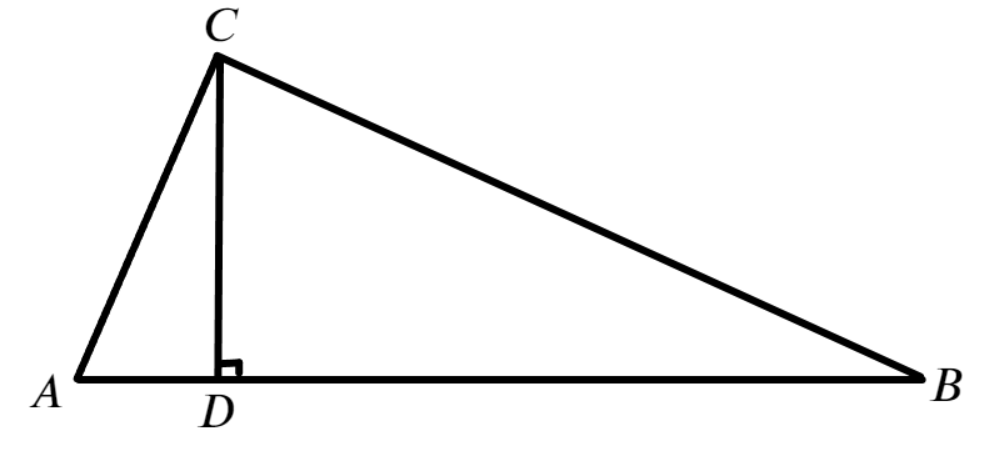
\includegraphics[scale=0.35]{g8-219b.png}}
\end{figure}\\
Если $CD^2=AD\cdot DB,$ то $\cfrac{CD}{AD}=\cfrac{DB}{CD}$ и треугольники $CDB$ и $ADC$ подобны по двум сторонам и углу между ними $(\angle ADC=\angle BDC=90^\circ).$ Тогда $\angle B=\angle ACD=90^\circ-\angle A,$ поэтому $\angle C=180^\circ-\angle A-\angle B=90^\circ,$ ч.т.д.\\
б) \begin{figure}[ht!]
\center{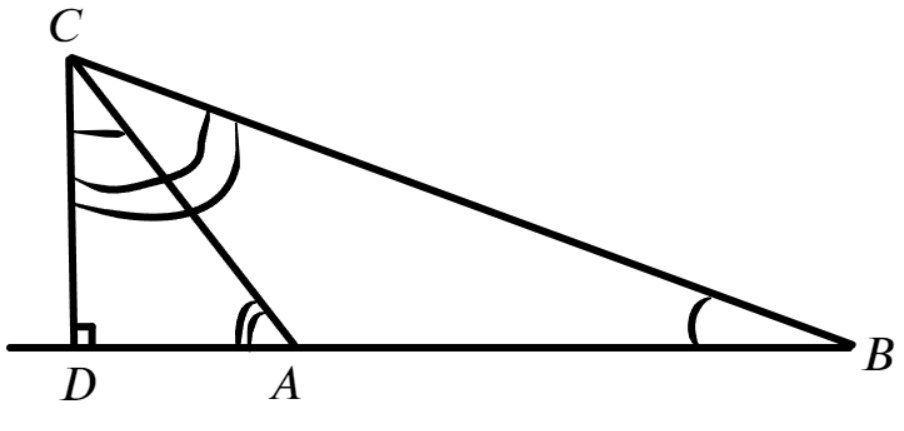
\includegraphics[scale=0.35]{g8-219.png}}
\end{figure}\\
Если взять $\angle A=110^\circ,\ \angle B=20^\circ,\ \angle C=50^\circ,$ то те же треугольники, что и в пункте а), будут подобны и соотношение также будет выполняться.\\
